% Preamble
\documentclass [a4paper,12pt,oneside,final,titlepage]{article}
\usepackage[left=35mm,top=35mm,right=26mm,bottom=10mm]{geometry}

\usepackage{listings}
\usepackage{graphicx}
\usepackage{color}
\usepackage{float}
%\usepackage{natbib}
\usepackage{fancyhdr}
\usepackage{pdfpages}
\usepackage[toc,page]{appendix}
%\usepackage{biblatex}
\usepackage{cite}
\usepackage{url}
%\addbibresource{biblio.bib}


\pagestyle{fancy}
%\fancypagestyle{IHA-fancy-style}{%
  \fancyhf{}% Clear header and footer
  \fancyhead[LE,LO]{Hessler}
  \fancyhead[RO,RE]{Page \thepage}
%  \fancypagestyle{plain}{\pagestyle{fancy}}
%  %\fancyfoot[C]{\thepage\ of \pageref{LastPage}}% Custom footer
%  \renewcommand{\headrulewidth}{0.0pt}% Line at the header visible
%  \renewcommand{\footrulewidth}{0.4pt}% Line at the footer visible
%%}



\definecolor{dkgreen}{rgb}{0,0.6,0}
\definecolor{gray}{rgb}{0.5,0.5,0.5}
\definecolor{mauve}{rgb}{0.58,0,0.82}
\definecolor{grey}{rgb}{0.9,0.9,0.9}

%\setcounter{topnumber}{2}
%\setcounter{bottomnumber}{2}
%\setcounter{totalnumber}{4}
%\renewcommand{\topfraction}{0.85}
%\renewcommand{\bottomfraction}{0.85}
%\renewcommand{\textfraction}{0.15}
%\renewcommand{\floatpagefraction}{0.8}
%\renewcommand{\textfraction}{0.1}
%\setlength{\floatsep}{5pt plus 2pt minus 2pt}
%\setlength{\textfloatsep}{5pt plus 2pt minus 2pt}
%\setlength{\intextsep}{5pt plus 2pt minus 2pt}


\lstset{frame=tb,
  language=Java,
  aboveskip=3mm,
  belowskip=3mm,
  showstringspaces=false,
  columns=flexible,
  basicstyle={\small\ttfamily},
  numbers=none,
  numberstyle=\tiny\color{gray},
  keywordstyle=\color{blue},
  commentstyle=\color{dkgreen},
  stringstyle=\color{mauve},
  breaklines=true,
  breakatwhitespace=true,
  tabsize=3
}
\lstset{frame=tb,
  language=C++,
  aboveskip=3mm,
  belowskip=3mm,
  showstringspaces=false,
  columns=flexible,
  basicstyle={\small\ttfamily},
  numbers=none,
  numberstyle=\tiny\color{gray},
  keywordstyle=\color{blue},
  commentstyle=\color{dkgreen},
  stringstyle=\color{mauve},
  breaklines=true,
  breakatwhitespace=true,
  tabsize=3
}
\lstdefinestyle{numbers} {numbers=left, stepnumber=1, numberstyle=\tiny, numbersep=10pt}
\lstdefinestyle{MyFrame}{aboveskip=3mm,
  belowskip=3mm,
  showstringspaces=false,
  columns=flexible,
  basicstyle={\small\ttfamily},
  numbers=none,
backgroundcolor=\color{grey},
  numberstyle=\tiny\color{gray},
  keywordstyle=\color{blue},
  commentstyle=\color{dkgreen},
  stringstyle=\color{mauve},
  breaklines=true,
  breakatwhitespace=true,
  tabsize=3,frame=shadowbox}
\lstdefinestyle{C++Style} {language=C++,style=numbers,style=MyFrame,frame=lines}
\lstdefinestyle{JavaStyle} {language=Java,style=numbers,style=MyFrame,frame=lines}


\setlength{\voffset}{-0.5in}

\title{An Implementation of Java Native Interface (JNI) to Replace a Socket}
\author{Brandon Hessler  \\
	Penn State - World Campus  \\
	Enterprise Integration \\
	SWENG568 Section 1 \\
	Program: Software Engineering M.S. \\
	}

\date{\today} 

\begin{document}
	\maketitle
	\tableofcontents
	\newpage
	\section{Project Introduction}
	The integration of applications is essential to the world we live in today. As programmers and software engineers we cannot effectively work or deliver the services necessary for our businesses or industries without integrating applications and systems together. With the world becoming more and more integrated and automated, the techniques that we learned in this course become more and more valuable.\\

On to my project. At work, I work on an application named TADA\footnote{Test Activity Data Aggregator} that needs to integrate with another application, the AP\footnote{Attenuator Program} that controls signal attenuator switch boxes. Originally, we wanted my Java program to run the switch boxes outright but there was an issue of a lot of logic that went into the code for the program and not wanting to completely rewrite it. Plus, this issue was compounded by a classification issue that could arise in some situations: with that we decided on a connection between the two. Myself and the other programmer who integrated these three years ago did not know of an other ways to communicate between two programs other than sockets. We came up with the ICD\footnote{Interface Control Document} shown in appendix \ref{appendix:icd}. With these messages, I would send him one of these messages and his program (the AP) would either set the value I gave to him or respond with the requested values. \\


	\subsection{Business View of the Integration Needs }
	From the perspective of the business, these applications need to work together to provide the test engineers both information of the results of a test as well as let them control the attenuation of the signals during the test. With these tools integrated it will not only save money with the ability to have less people working during a test event, but will give greater figelity to the data collected. In my program, I am able to calculate what the result of the test is, but without the ability to collect the results straight from the AP during the test, we are unable to make the best test taking decisions that we can in real time. Instead of using sockets, the JNI\footnote{Java Native Interface} will allow us to not have the AP running during the test and instead will allow us to call the code already written in the AP from the TADA program. 

	
	\section{Workflows or Process Flows Design (e.g., Integration logic across integrated applications)}
	The nice thing about using JNI in this context is that from my Java program I can do all of the initialization that is needed for the AP. There is no need to open up the AP as an application but we can instead use its functionalities as a background process of TADA. This means I do not have to make calls to the hardware directly, which would be hard since there are no Java drivers for that product so I would have to write them myself.
	\subsection{Data Flow}
The data flow for this integration can be seen in figure \ref{fig:data}. This shows that TADA is making a call to the AP which will then in turn poll either of the attenuator switch boxes, and then return that data back to TADA, if asked. Some of the commands, like setting the Scan Rate (see message ID 15 in appendix \ref{appendix:icd}, are for the AP to regulate how often to tell the switch boxes to change. This flow of data may mean that the AP is not going to give that message to the switch boxes, but will give an entirely different one at the interval it was told to.
	\begin{figure}[htp]
		\centering
		\includegraphics[height=55mm]{dataFlow}
		\caption{Shows the flow of data between TADA and the AP}
		\label{fig:data}
	\end{figure}

	\subsection{Control Flow}
Probably the most convenient feature of the JNI implementation is that the control will stay with the program that was originally designed to do so. The control will originate from TADA, but once a run is started, the AP will have control over the switch box hardware and will constantly be away of their values. From TADA I will be able to query those values whenever I need them from the AP. The control flow can be seen in figure \ref{fig:control}.
	\begin{figure}[htp]
		\centering
		\includegraphics[height=55mm]{controlFlow}
		\caption{Shows the control flow TADA, the AP, and the switch box hardware}
		\label{fig:control}
	\end{figure}

	\section{Integration Design (i.e., Approach to implementing the identified integration logic)}
	At a high level this integration should be fairly easy, remove the socket connection from my code in TADA and replace it with the JNI code. From The Breakfast Post website \cite{jniWebsite} I looked at his step by step instructions on how to create JNI code and the C wrapper required to run it. Now all I needed to do was learn a bit of C and C++. The steps for the JNI and its wrapper seem to be fairly straightforward. 
\begin{enumerate}
	\item Find methods and classes that are to be called in the C++ code\\
Ensure calls needed to make in C++ are public.
	\item Make corresponding classes or methods within the Java code \\
These must be identified in the code as native. You then leave those methods empty since the code that will be called will be from the C++ code.
	\item Create the JNI wrapper in C \\
This will correlate the Java code and methods to the C++ code and methods. It seems that using JNI is more writing in C than it is in Java.
	\item Test code
\end{enumerate}

%This is where I need to start coding and identifying the classes that need to be used
	\subsection{Architecture Model}
	As you can see in figure \ref{fig:overview} the JNI process is a fairly straightforward way to cross the gap between Java and C++ code. The only middle process required is that of the JNI wrapper. Note that this is not the entire architecture of both systems as those are both irrelevant to this discussion and also I am unable to give that out in this venue. The AttenuatorDriver is part of the Attenuator Program and its code is not given here as it is the property of the Navy and I am not able to distribute it. In \ref{fig:overview} you will notice the colors of the lines. The red path is that for the real system that we are going to integrate this at work, the blue is the one for this project, and the purple path is the one followed in either case. 
	\begin{figure}[htp]
		\centering
		\includegraphics[height=90mm]{overview}
		\caption{The architecture model of the JNI bridge between the applications}
		\label{fig:overview}
	\end{figure}

	\subsection{Functional Model}
	In this functional model (figure \ref{fig:functional}) you can see the functions that are implemented. You will notice that I am replacing all of the socket calls that were previously made via the byte arrays in appendix \ref{appendix:icd} as well as the calls for the AP to connect to the attenuator switch boxes. These switch boxes connect via socket, using IP address and port, to the AP using always localhost as the address and ports 5150 and 5151 for boxes one and two, respectively. As you will see in the code soon, I am writing the functions to take in a port just in case those change out of necessity, but they will be hard coded in a \emph{constants} file in case later we need to ask the user's input; it would be easier to do that later on the Java side then to go back into the JNI code.
	
	\begin{figure}[htp]
		\centering
		\includegraphics[height=80mm]{Packages}
		\caption{The functional model of the JNI bridge function calls}
		\label{fig:functional}
	\end{figure}

\section{Implementation and Programming}
	\subsection{Classes Used}
	With the code that I am writing for this section I will include the following files and their purposes.
	\begin{enumerate}
		\item Java Classes
			\begin{enumerate}
				\item Main.java - Launches the GUI\footnote{Graphical User Interface}
				\item AttenuatorControl.java - GUI for the control of the attenuator functions. Some of these will be automated later but this will be useful for testing.
				\item AttenuatorJni.java - This will contain the JNI calls that will call the code from the other application
				\item AttenuationPower.java - Makes it easier for the program to output good java values from the JNI call \emph{getData()}
				\item AttenuationValue.java - Makes it easier for the program to output good java values from the JNI call \emph{getAttenuationValues()}
				\item RegExFieldFormatRestrictor.java - This is a class that extends Document that makes it easy to apply a regular expression to a JTextField for input validation (or in this case restriction). A coworker and I wrote this at work.
			\end{enumerate}
		\item C++ Classes
			\begin{enumerate}
				\item AttenuatorSimulator.cpp -  Returns the appropriate values for the information given form the Java GUI
				\item AttenuatorSimulator.h -  Header File for above
				\item AttenuatorJniWrapper.cpp - This is the C++ file containing the code of the JNI wrapper, this is the bridge between the C++ code and the Java code
				\item AttenuatorJniWrapper.h - This is the header file for the JNI wrapper 
			\end{enumerate}
	\end{enumerate}
	
	
	For this section I will explain the code that I needed to write to accomplish the communication from Java to C++ without the use of sockets. I will be explaining them from the front to the back end of the code, starting from the user interface and working back to the simulated hardware program (written in C++) which in practice will communicate with the hardware itself.

\subsection{Java Code}
	\begin{figure}
		\centering
		\includegraphics[height=110mm]{gui}
		\caption{The graphical user interface of the test program}
		\label{fig:gui}
	\end{figure}

	Starting with the Java element, I wrote a mock-up of the GUI. In the final product, many of these processes would not necessarily have a button associated with it, but for testing purposes it made sense to make a button for each of the function calls necessary. Figure \ref{fig:gui} is a screenshot of that GUI. The full code written will not be shown here but is available with this document as are the classes \emph{AttenuationPower.java} and \emph{AttenuationValue.java} since that code is altogether standard. The only part of the GUI code I will show is the part that uses the RegExFieldFormatRestrictor and that is so you are not confused when you try to type wrong values in the JTextFields (Listing \ref{lst:RegEx}). I did get the code for the port number regular expression from StackOverflow \cite{regex}. The code that makes the JNI calls though is important to include here and is shown below in Listing \ref{lst:AttenuatorJni}. This shows that here we are making the \emph{native} calls that will be calling the methods from the AttenuatorJniWrapper dll that is included in the Java project; the details of which I will explain now. 

	\begin{figure}[htp]
		\centering
		\includegraphics[height=40mm]{help}
		\caption{The help dialog that gives the tester hints on how to use this properly}
		\label{fig:help}
	\end{figure}	
	\lstinputlisting[style=JavaStyle,caption={AttenuatorControl RegEx}, label={lst:RegEx}, firstline=165, lastline=175]{AttenuatorControl.java}

	%\begin{lstlisting}[style=JavaStyle]
	\lstinputlisting[style=JavaStyle, caption={AttenuatorJni Java native code}, label={lst:AttenuatorJni}]{AttenuatorJni.java}

\subsection{C++ Code}
	The AttenuatorJniWrapper dll was created from the AttenuatorJniWrapper.cpp and AttenuatorJniWrapper.h files that I alluded to above. The AttenuatorJniWrapper.h file can be created or generated through the use of \textbf{javah}. The javah tool is executed via command line and turns a java file (in this case the AttenuatorJni.class) into a header file for use in JNI. Notice I said the .class file, not the .java file, this was something that I did not realize and took me about five hours to figure out why my commands in the command line were not working. These files, along with the AttenuatorSimulator.lib file, form the bridge between the simulator and the Java code (and GUI). As you can see below in Listing \ref{lst:Wrapper} this code takes calls from the Java code, calls the C++ code (the attenuator simulator), then translates the C++ object types into Java objects that can be returned, then returns them to Java. Since all of the necessary information can be gained through looking at just the .cpp file, I will not clutter this paper further with the .h file.

	\lstinputlisting[style=C++Style,caption={AttenuatorJniWrapper code}, label={lst:Wrapper}]{AttenuatorJniWrapper.cpp}

	To make the AttenuatorJniWrapper class work it needs to know what C++ calls to make, that is why I had to include the AttenuatorSimulator.lib file in the project (or at least link the project to it). That static library was created from the AttenuatorSimulator.h and .cpp files. These files have a few basic variables that do not do much other than verify that all of the calls coming from the Java code are working, the values given are valid, and the calls made are valid. I will only show a few lines of the AttenuatorSimulator.h file (Listing \ref{lst:Simh}) since I declare a few things that are necessary to the .cpp file, but most everything of note is in the .cpp file. 

	\lstinputlisting[style=C++Style, caption={AttenuatorSimulator global variables}, label={lst:Simh}, firstline=1, lastline=20]{AttenuatorSimulatorVS.h}

This .cpp file (Listing \ref{lst:simcpp}) shows the validation that the program would use before trying to send signals to the signal attenuator switch boxes such as to ensure that they are running before telling them to stop and only allowing them to pause their steps if they are already running. Otherwise, this class is returning false values that would usually be reserved for the actual values that the hardware is set to. 

	\lstinputlisting[style=C++Style, caption={AttenuatorSimulator end code}, label={lst:simcpp}]{AttenuatorSimulatorVS.cpp}

	%\end{lstlisting}
	\newpage
	\section{Bibliography}
	\bibliography{biblio}{}
	\bibliographystyle{apalike}
	\newpage
	\begin{appendices}
		\section{Previous ICD}
		\label{appendix:icd}
		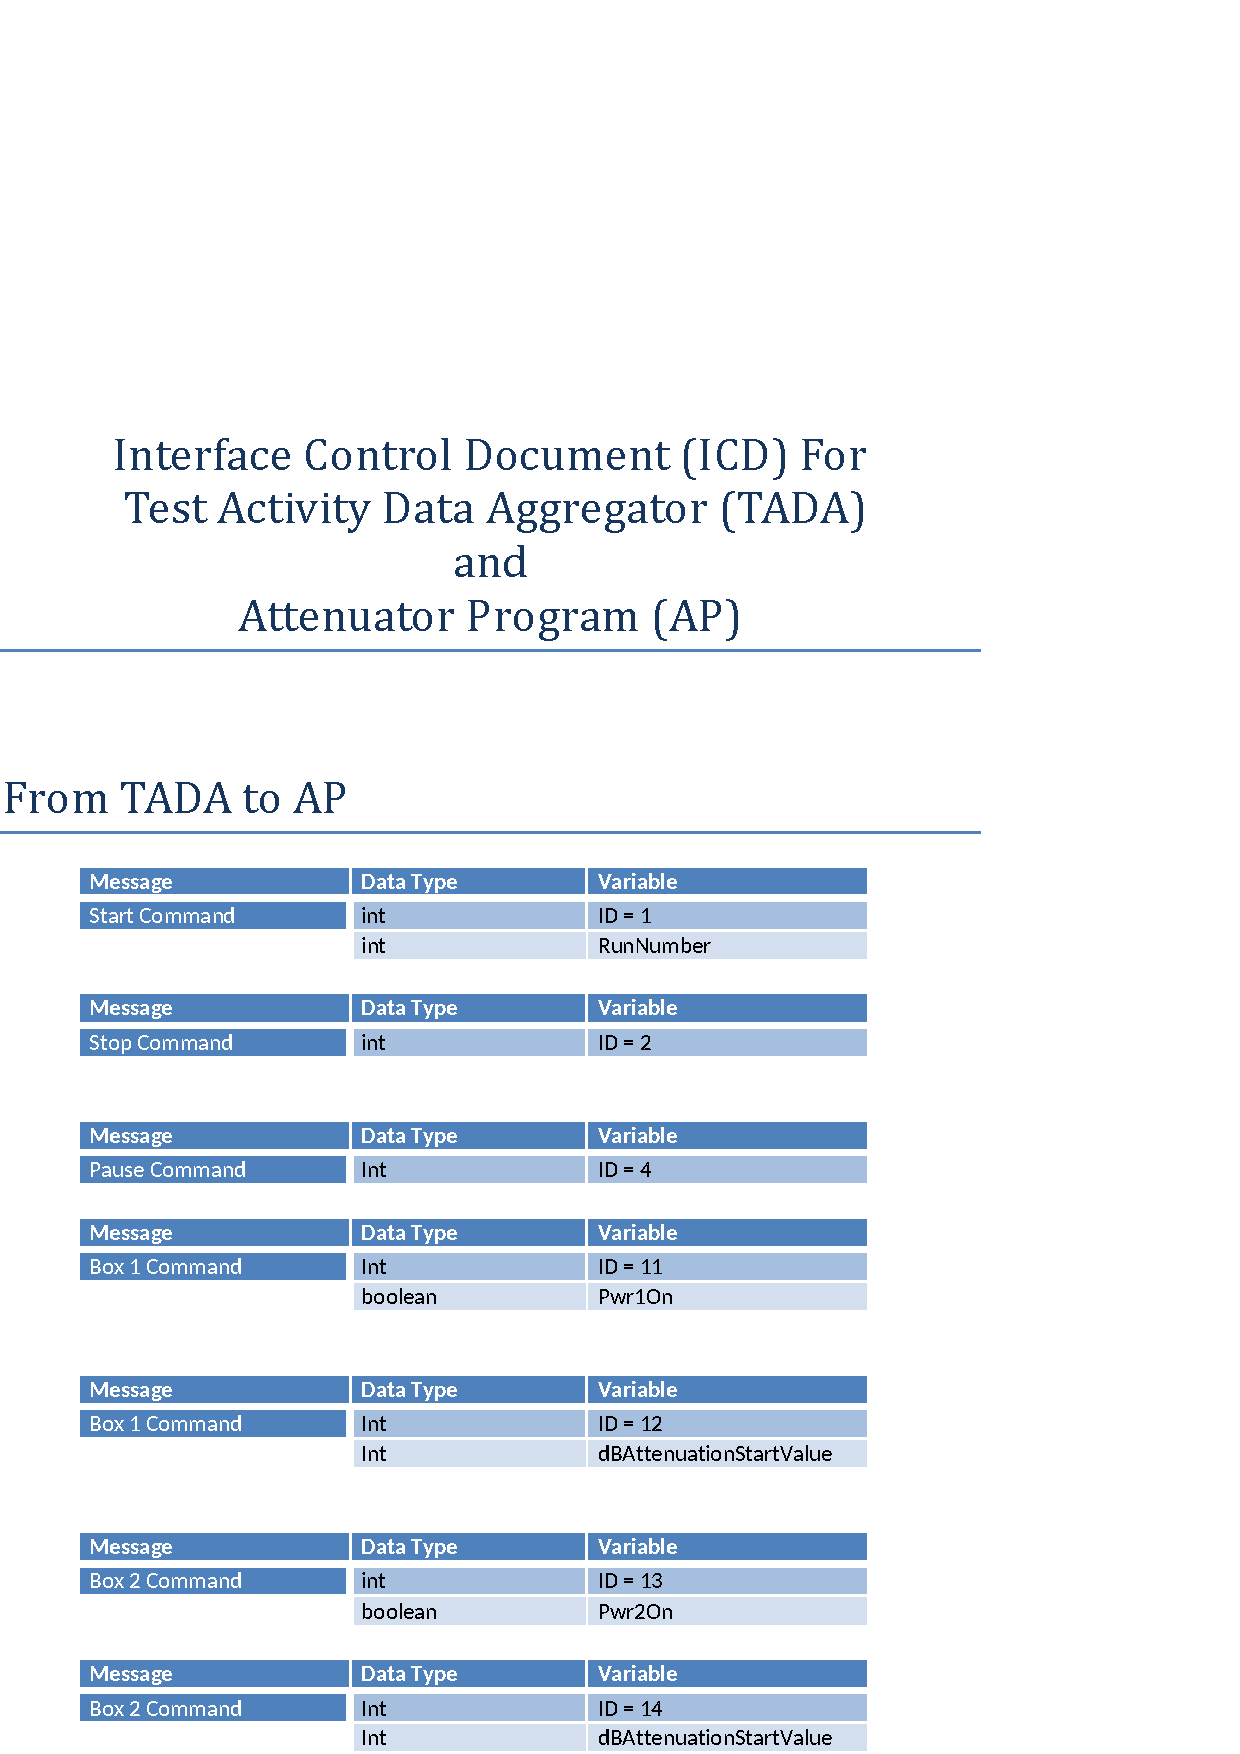
\includepdf[pages=-, pagecommand={\pagestyle{fancy}}]{TADA-AP-ICD.pdf}
	\end{appendices}	


	

	
	
\end{document}